\documentclass[letterpaper,12pt]{article}
\usepackage{tabularx} % extra features for tabular environment
\usepackage{amsmath}  % improve math presentation
\usepackage{float}
\usepackage{pdfpages}


\usepackage{graphicx} % takes care of graphic including machinery
\graphicspath{ {./figures/} }
%\usepackage[margin=1in,letterpaper]{geometry} % decreases margins
%\usepackage{cite} % takes care of citations
\usepackage[final]{hyperref} % adds hyper links inside the generated pdf file
\hypersetup{
	colorlinks=true,       % false: boxed links; true: colored links
	linkcolor=blue,        % color of internal links
	citecolor=blue,        % color of links to bibliography
	filecolor=magenta,     % color of file links
	urlcolor =blue         
}
\usepackage[margin = 1in,headsep=0.5cm,headheight=2cm,letterpaper]{geometry} 

\usepackage{fancyhdr}
\pagestyle{fancy}
\lhead{Student 1 : Ahmet Akman 2442366 \\ Student 2: Yusuf Toprak Yıldıran 2444149 \\ Assistant: Onur Selim Kılıç}
\rhead{Date: \today \\ Group: Wednesday Morning - 5} 
%\cfoot{center of the footer!}
\renewcommand{\headrulewidth}{0.1pt}



\begin{document}
\thispagestyle{empty}

\title{Spring 2022 EE214 Project Work  \protect\\ PreliminaryWork }
\author{Ahmet Akman 2442366 \protect\\ Yusuf Toprak Yıldıran 2444149 \protect\\ Assistant: Onur Selim Kılıç}
\date{\today}
\maketitle
\tableofcontents
%\begin{abstract}
%abstract
%\end{abstract}
\section{Introduction}
\section{Experimental Results and Discussion}
The results of the experiment are discussed in the following steps.
%
\subsection{Transmitter Unit}
\subsection{Receiver Unit}
In this part a receiver needed to be designed. So, let us first define the design requirements.
\begin{itemize}
    \item The receiver should be able extract the desired signal amongst the signals with 12 different frequencies.
    \item The receiver should be able make a difference between the needed signal and others at least 10dB. (Closely related to the Q factor.)
    \item The receiver should provide option of channel adjustment with (at most) 2 potentiometer. Adjustment with 1 pot is the target. 
\end{itemize}
In order to design a receiver unit that satisfies the fundamental requirements specified above, a circuit that only allows the signal with desired frequency to pass neeeded to be constructed. So , a filter design is expected which act like as a fourier transformer. There are passive and active filter designs which allows to pass below (low pass) or above (high pass) thereshold frequencies. By combining those two filters one can build a filter which allows only certain band of signals. This is called band pass filter.
\begin{figure}[H]
    \centering
    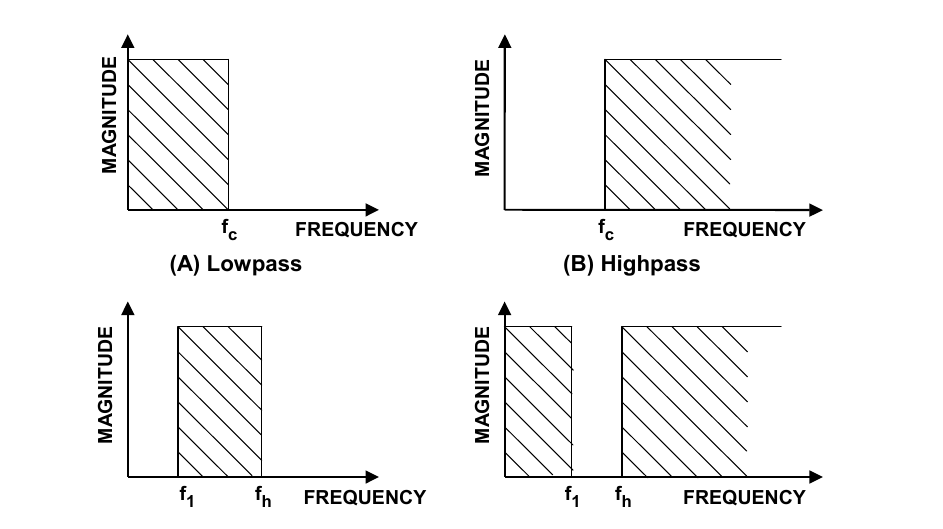
\includegraphics[width = 0.75\textwidth]{bandpass.png}
    \caption{Filter Responses (ideal)}
\end{figure} 
Passive filters are not considered here since they would not be feasable in an adjustable setup. The transfer function of band-pass filter can be explained as following.
\[
H(s) = \frac{H_0 (\omega_0)^2}{s^2 + \frac{\omega_0}{Q} s  + (\omega_0)^2}    
\]

Now let us examine briefly transfer responses in the literature to choose an optimum design path.
\subsubsection{Butterworth}
Butterworth transfer response offers clean pass and not-pass regions in other words no ripple. However, the band that allows the signals is not narrow.
\subsubsection{Chebyshev}
Chebyshev transfer response offers narrower band however it has ripples in the pass band.
\subsubsection{Bessel}
Bessel filter is optimized to obtain better transient response due to a linear phase (i.e.
constant delay) in the passband.

\vspace{4mm}
For our case as long as it is tuned carefully all three transfer responses can be used. However in order to have  better frequency discrimination Chebyshev function is selected to be used in this phase of the project. The values for the Chebyshev function will be fetched from the design tables available in internet. (The table is not included here in order not to excess page limit.)
\\

\vspace{4mm}
Now let us examine briefly the available design topologies to choose which design path to go for.
\subsubsection{KHN Filter ( State Variable Filter)}
\subsubsection{Sallen-Key Band Pass}
\subsubsection{Multiple Feedback Band Pass}



\subsection{Speaker Unit}

\section{Conclusion}
\section*{Appendix A}


\end{document}

%%%%%%%%%%%%%%%%%%%%%%   EXAMPLE TABLE   %%%%%%%%%%%%%%%%%%%%%%%%%%%%%%%%
\begin{table}[H]
\begin{center}
    \caption{Resistance reading by color code convention.}
    \vspace{2mm}
    \begin{tabular}{||c | c | c||} 
        \hline
        Color Order & Value & Tolerance \\ [0.5ex] 
        \hline\hline
        Brown / Black / Red / Gold & 1k\( \Omega \) & \( \% \) 5  \\ 
        \hline
        Yellow / Violet / Red / Gold & 4.7k\( \Omega \) & \( \% \) 5   \\
        \hline
        Brown / Grey / Orange / Gold & 18k\( \Omega \) & \( \% \) 5  \\ [1ex] 
        \hline
    \end{tabular}
\end{center}
\end{table}


%%%%%%%%%%%%%%%%%%%%%%   EXAMPLE IMAGE   %%%%%%%%%%%%%%%%%%%%%%%%%%%%%%%%
\begin{figure}[H]
\centering
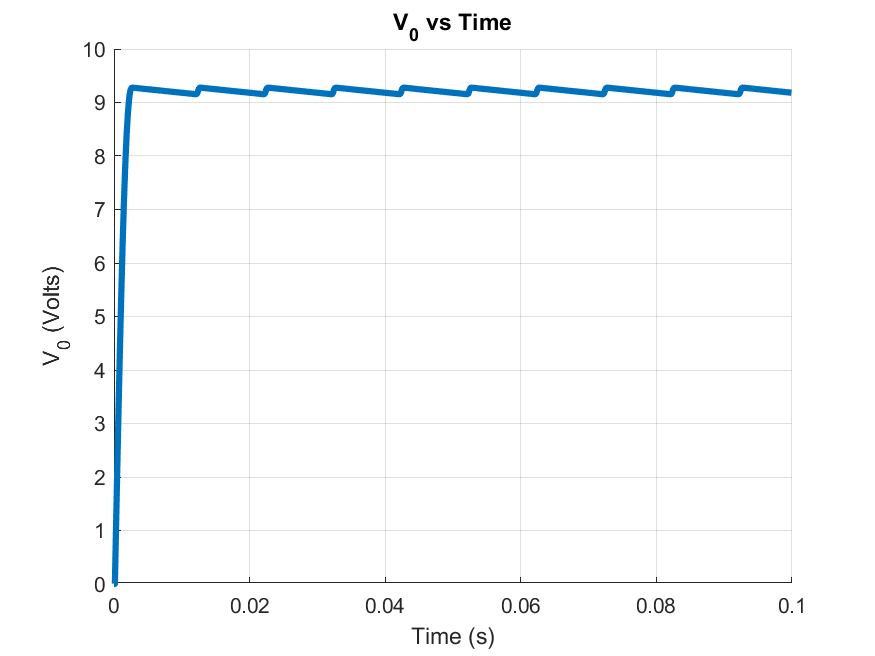
\includegraphics[width = 0.75\textwidth]{5.png}
\caption{Circuit schematic for the step 5}
\end{figure} 

%%%%%%%%%%%%%%%%%%%%%%   EXAMPLE IMAGE FROM PDF   %%%%%%%%%%%%%%%%%%%%%%%%%%%%%%%%
\begin{figure}[H] \centering{
	\includegraphics[scale=0.25]{2a_plot.pdf}}
	\caption{Experiment 2}
\end{figure}
%%%%%%%%%%%%%%%% Deneme Push